\chapter{Realisierung}

\section{Technische Erkenntnisse}

\subsection{Blöcke auf dem Chip}
Durch Auslesen mehrerer ausgeliehenen Büchern und dem Abgleich mit der erhaltenen Datenbank von der Speicherbibliothek, wurde herausgefunden, dass die Blöcke null bis drei die für die Buch-ID relevanten Informationen enthalten (siehe Tabelle \ref{tbl:ListeBloecke} und Abbildung \ref{fig:AusgeleseneBloeckeUndBarcode}). Weiter werden für die ID des Buches nur darstellbare Unicode-Charaktere verwendet und nicht der geschriebene Hex-Code.

\begin{table}[htb]
	\begin{tabularx}{\textwidth}{|l|l|l|X|}
		\hline
		\textbf{Blocknummer} & \textbf{Inhalt (Hex)} & \textbf{Inhalt (UTF8)} & \textbf{Beschreibung}\\
		\hline
		0 & 11010149 & I & Erster Block der BuchID \\
		\hline
		1 & 4c554d33 & LUM3 & Zweiter Block der BuchID \\
		\hline
		2 & 39303031 & 9001 & Dritter Block der BuchID \\
		\hline
		3 & 31333300 & 133 & Vierter Block der BuchID \\
		\hline
		4 & 00000081 &  & \\
		\hline
		5 & 3e43484c & >CHL & \\
		\hline
		6 & 55485349 & UHSI & \\
		\hline
		7 & 00000000 & - & Leerer Block \\
		\hline
		8 & 00000000 & - & Leerer Block \\
		\hline
		9 & 00000000 & - & Leerer Block \\
		\hline
		10 & 00000000 & - & Leerer Block \\
		\hline
		11 & 00000000 & - & Leerer Block \\
		\hline
		12 & 00000000 & - & Leerer Block \\
		\hline
		13 & 00000000 & - & Leerer Block \\
		\hline
		14 & 00000000 & - & Leerer Block \\
		\hline
		15 & 00000000 & - & Leerer Block \\
		\hline
		16 & 00000000 & - & Leerer Block \\
		\hline
		17 & 00000000 & - & Leerer Block \\
		\hline
		18 & 00000000 & - & Leerer Block \\
		\hline
		19 & 00000000 & - & Leerer Block \\
		\hline
		20 & 00000000 & - & Leerer Block \\
		\hline
		21 & 00000000 & - & Leerer Block \\
		\hline
		22 & 00000000 & - & Leerer Block \\
		\hline
		23 & 00000000 & - & Leerer Block \\
		\hline
		24 & 00000000 & - & Leerer Block \\
		\hline
		25 & 00000000 & - & Leerer Block \\
		\hline
		26 & 00000000 & - & Leerer Block \\
		\hline
		27 & 00000000 & - & Leerer Block \\
		\hline
	\end{tabularx}
	\caption{Blöcke und deren Inhalt für Beispiel HF RFID}
	\label{tbl:ListeBloecke}
\end{table}

\begin{figure}[p]
	\centering
	\begin{subfigure}[t]{.45\textwidth}
		\centering
		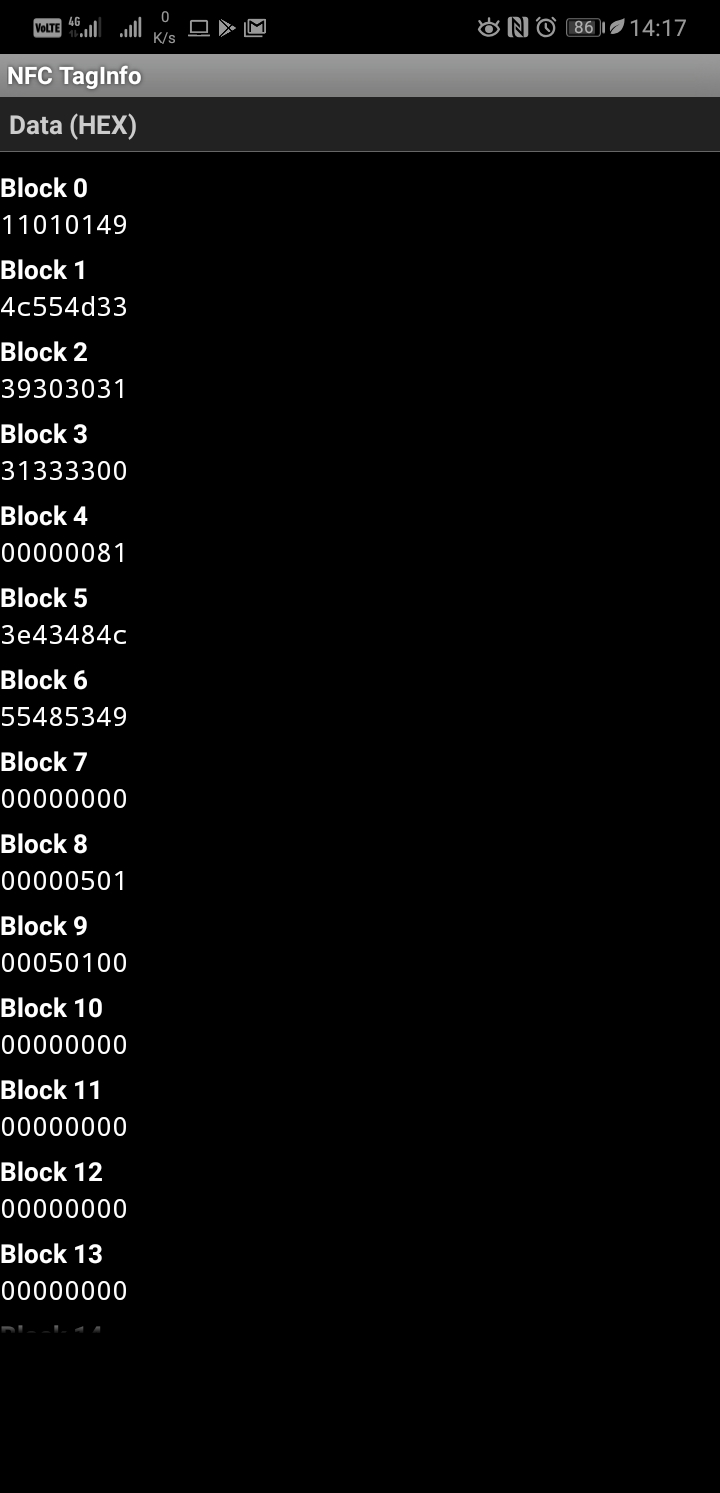
\includegraphics[keepaspectratio,width=\linewidth]{RFID_Blocks-Hex}
		\caption{Blöcke in Hex mit Smarphone ausgelesen}
	\end{subfigure}
	\begin{subfigure}[t]{.45\textwidth}
		\centering
		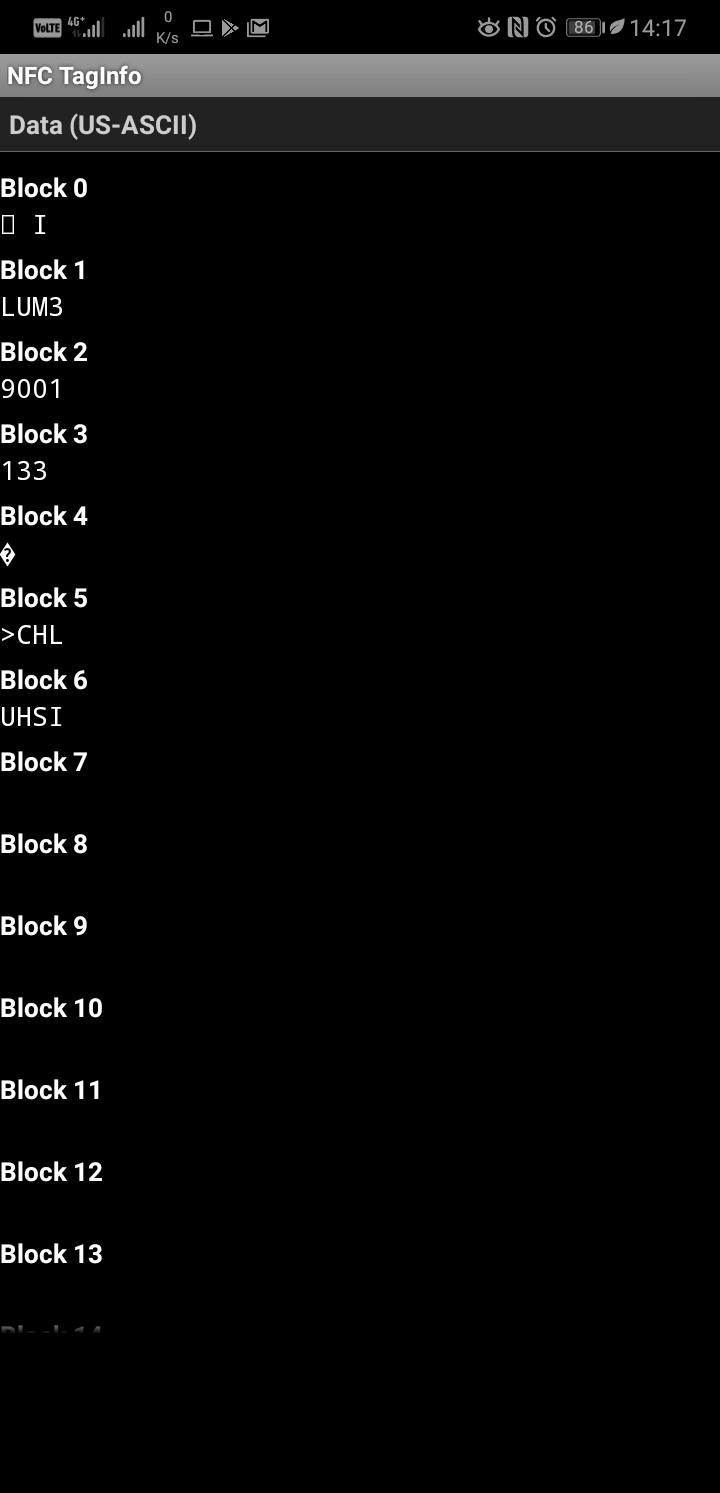
\includegraphics[keepaspectratio,width=\linewidth]{RFID_Blocks-Ascii}
		\caption{Blöcke in ASCII mit Smarphone ausgelesen}
	\end{subfigure}
	\begin{subfigure}[b]{.3\textwidth}
		\centering
		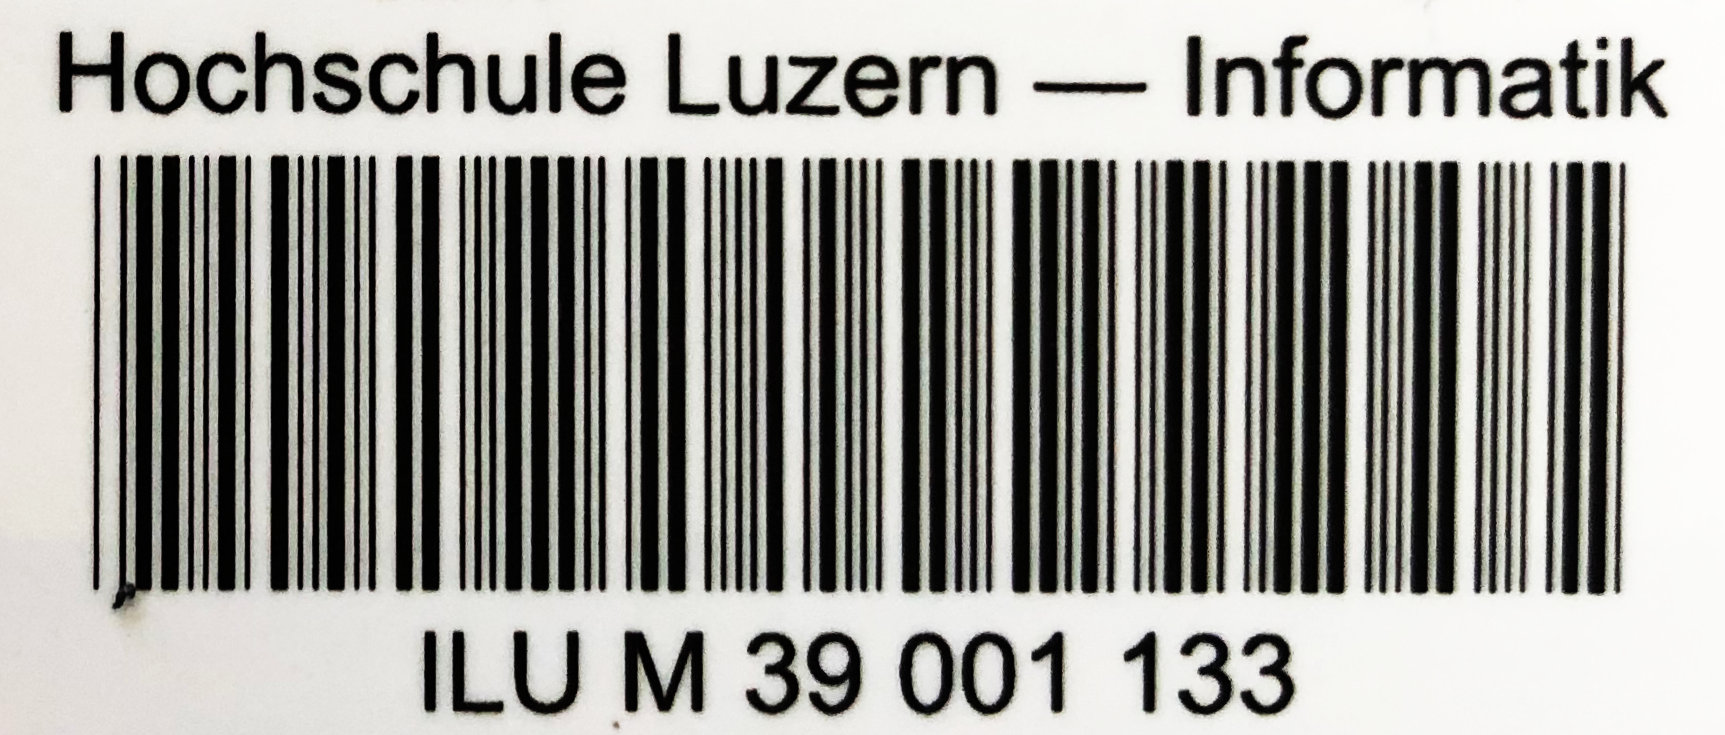
\includegraphics[keepaspectratio,width=\linewidth]{Barcode_BuchRFIDTag}
		\caption{Zugehöriger Barcode}
	\end{subfigure}
	\caption{Ausgelesene Blöcke und Barcode des Buches}
	\label{fig:AusgeleseneBloeckeUndBarcode}
\end{figure}


\clearpage
\section{Systemspezifikation Referenzimplementation}
\label{sec:SysSpec}

\subsection{Anforderungen}
\label{sub:ReferenzimplementationAnforderungen}
Hier werden die Anforderungen an die Referenzimplementation, welche bereits in Kapitel \ref{sub:Anforderungen} erwähnt wurden, nochmals aufgelistet.
\begin{legal}
	\item Die Referenzimplementation ist in der Lage die Buch ID eines Exemplares über RFID auszulesen.
	\item Die Referenzimplementation soll erkennen, wenn eine Box ein Exemplar (eines, welches mit RFID ausgestattet ist und technisch auch Lesbar ist) enthält, welches nicht dieser Box zugehörig ist.
	\item Die Referenzimplementation soll jede erkannte Unstimmigkeit (Exemplar, welches nicht zu diesem Behälter gehört) in einem Logdokument persistieren.
	\item Die Referenzimplementation soll in der Lage sein, dem Endbenutzer, in graphischer Form durch eine Konsolen-Ausgabe, mitzuteilen, welcher Behälter eine Unstimmigkeit enthält.
	\item Die Referenzimplementation soll die unter Laborbedingungen erhaltenen Resultate unter Realbedingungen verifizieren.
	\item Die Referenzimplementation soll mit einer Oracle Datenbank kommunizieren können.
\end{legal}

\subsection{Kontext}

Das nachfolgende Kontextdiagramm (Abbildung \ref{fig:Kontextdiagramm}) beschreibt die Interaktion der Referenzimplementation mit allen Umsystemen. Diese Umsysteme beinhalten den Benutzer, welche von der Referenzimplementation Informationen erhält, ein weiteres Umsystem beinhaltet ein Datenbankexport Dokument, welches dem System die Informationen zu einem Exemplar liefert. Das Letzte Umsystem ist die der RFID Reader, welches dar Referenzimplementation die Informationen eines gefundenen RFID Tags liefert.
\begin{figure}[htb]
	\centering
	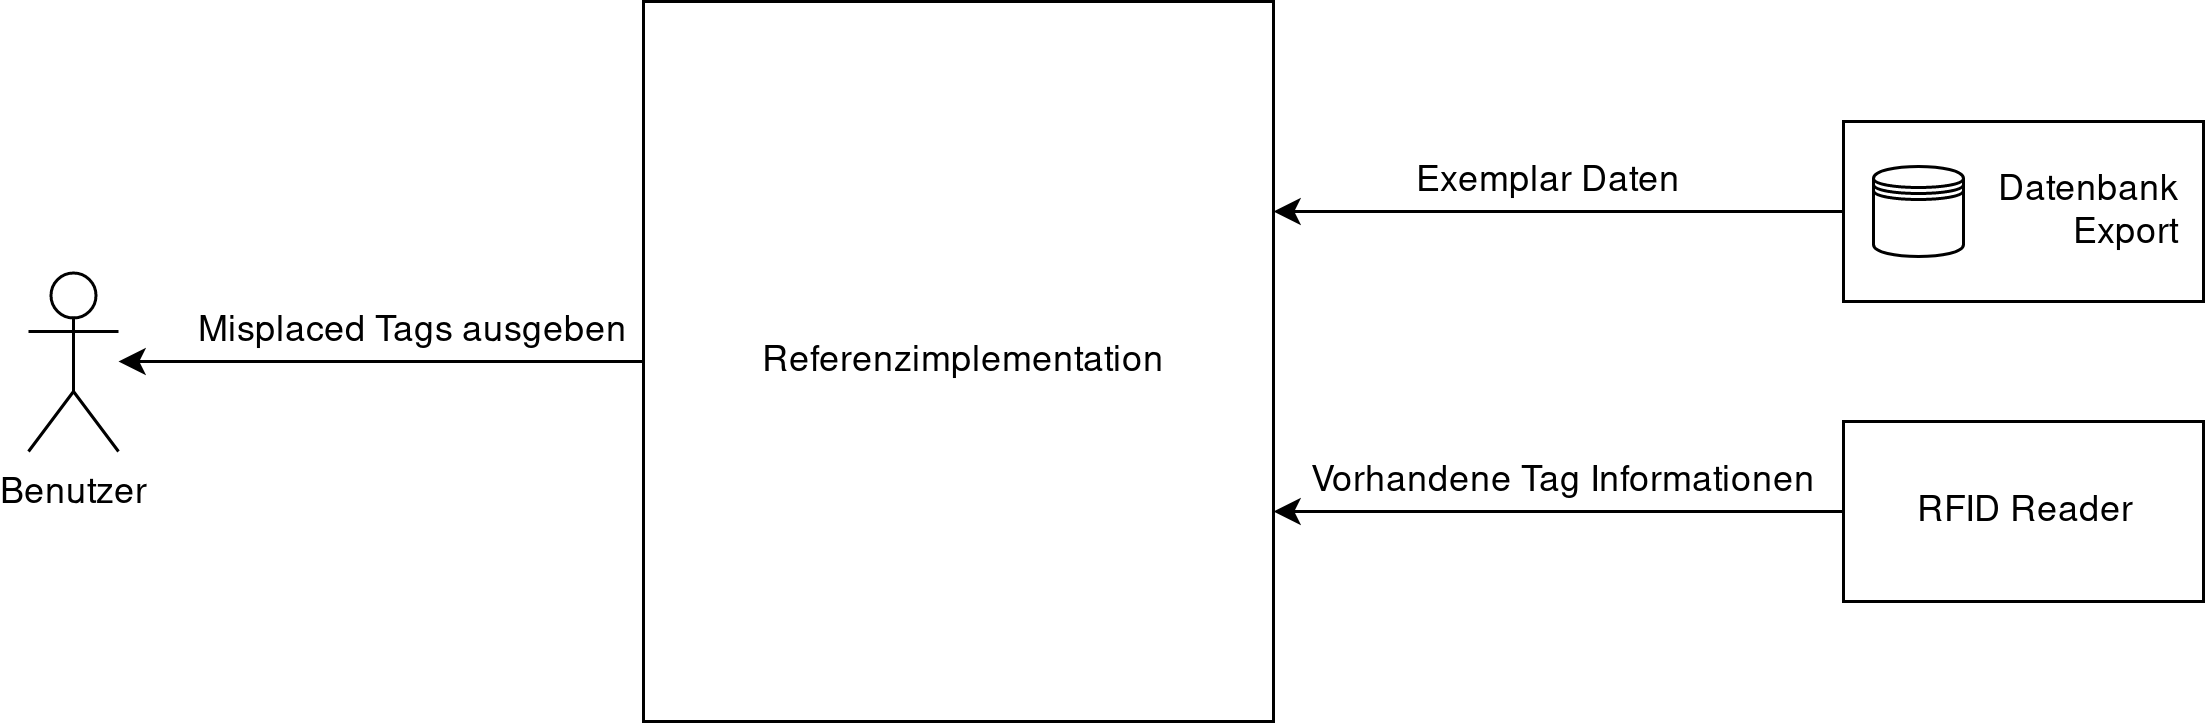
\includegraphics[keepaspectratio,width=.9\linewidth]{Kontextdiagramm}
	\caption{Kontextdiagramm der Referenzimplementation}
	\label{fig:Kontextdiagramm}
\end{figure}

\subsection{System}
\begin{figure}[htb]
	\centering
	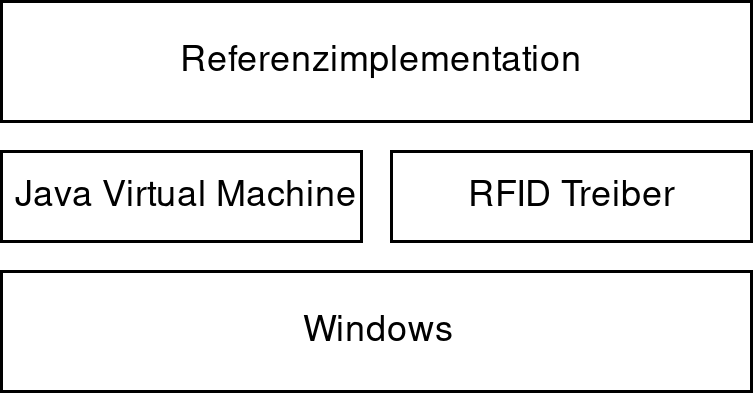
\includegraphics[keepaspectratio,width=.6\linewidth]{System}
	\caption{Darstellung der Systeme, von welcher die Referenzimplementation abhängt}
	\label{fig:System}
\end{figure}
\subsubsection{RFID Treiber}
Der verwendete RFID Treiber der Firma Hyientech setzt voraus, dass dieser auf einem Windows System läuft, in einer 32Bit Umgebung.

\subsection{Komponenten}
\begin{figure}[htb]
	\centering
	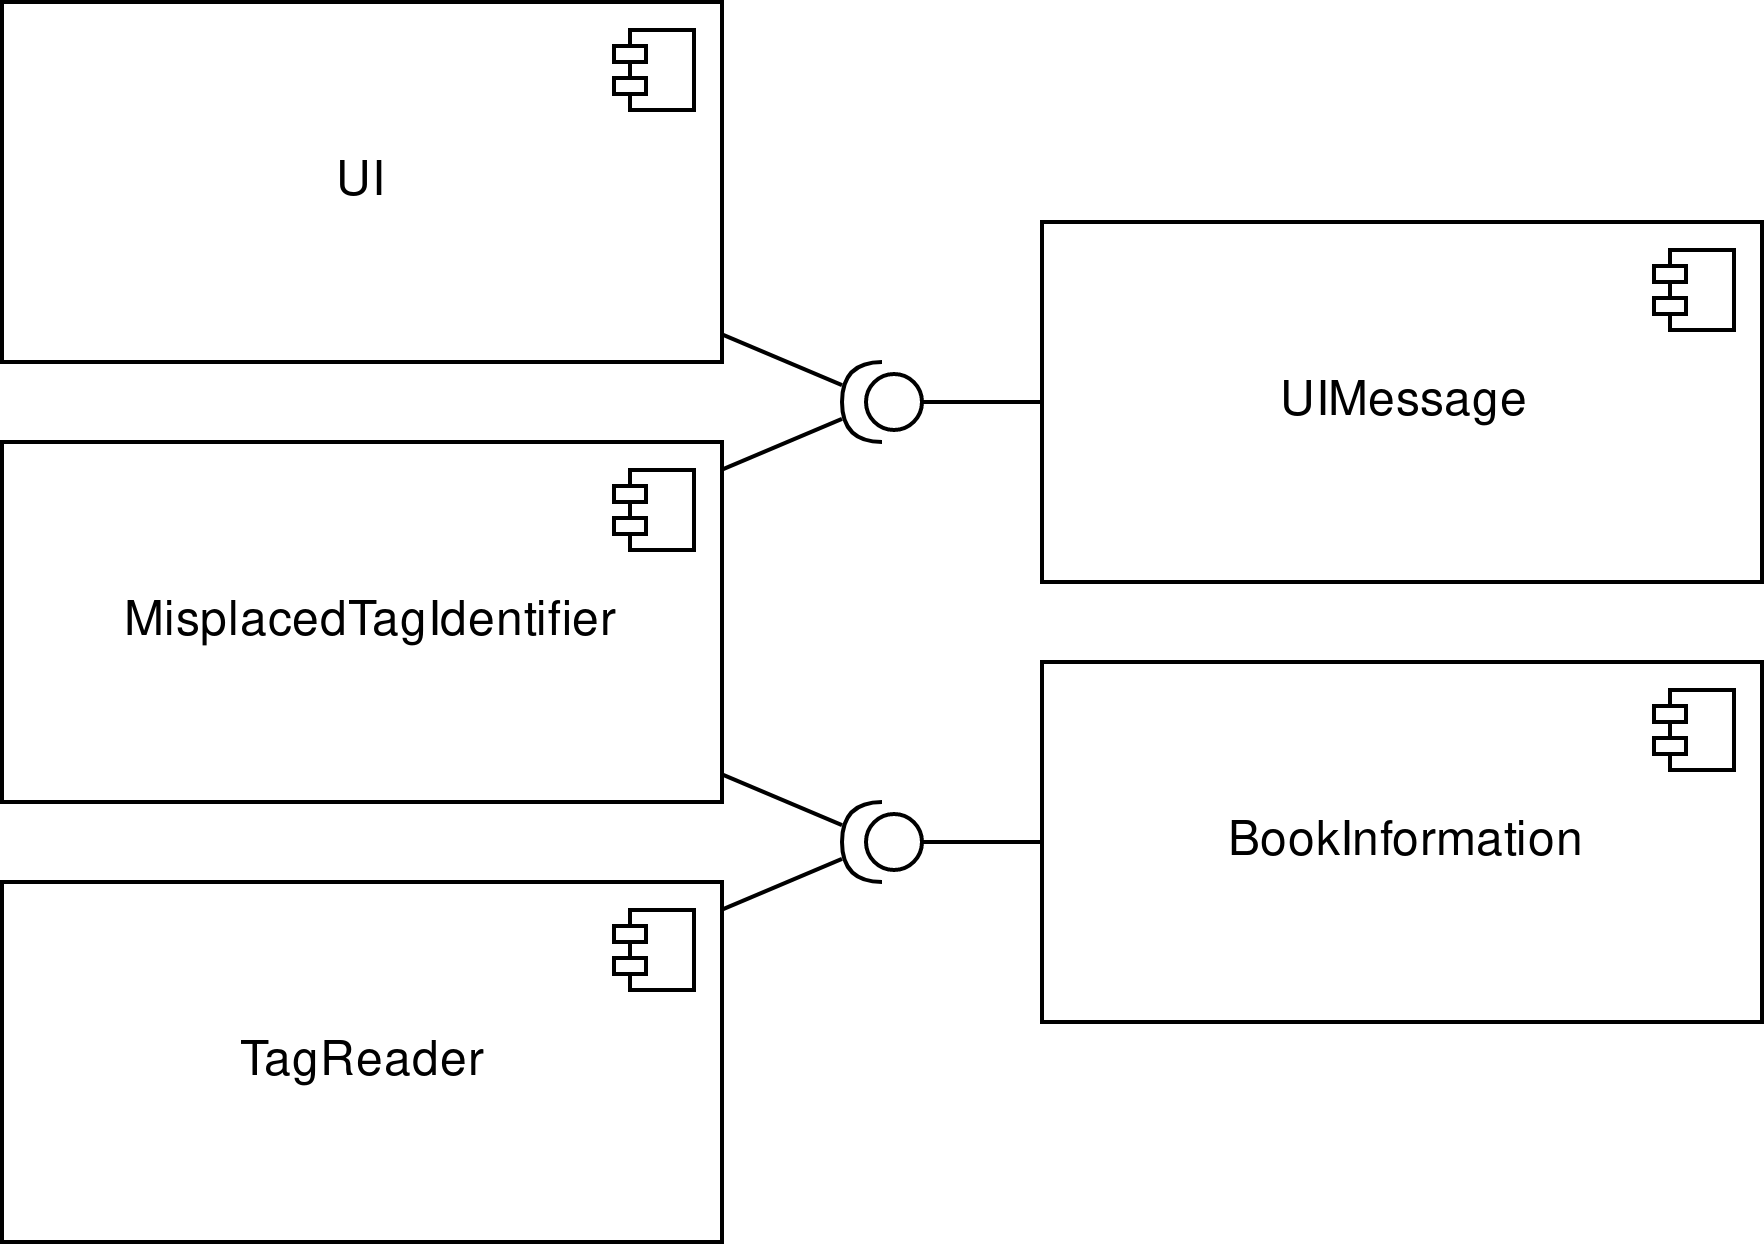
\includegraphics[keepaspectratio,width=.8\linewidth]{Komponentendiagramm}
	\caption{Darstellung der Klassen in der Komponente UI}
	\label{fig:Components}
\end{figure}

\subsubsection{UI}
\begin{figure}[htb]
	\centering
	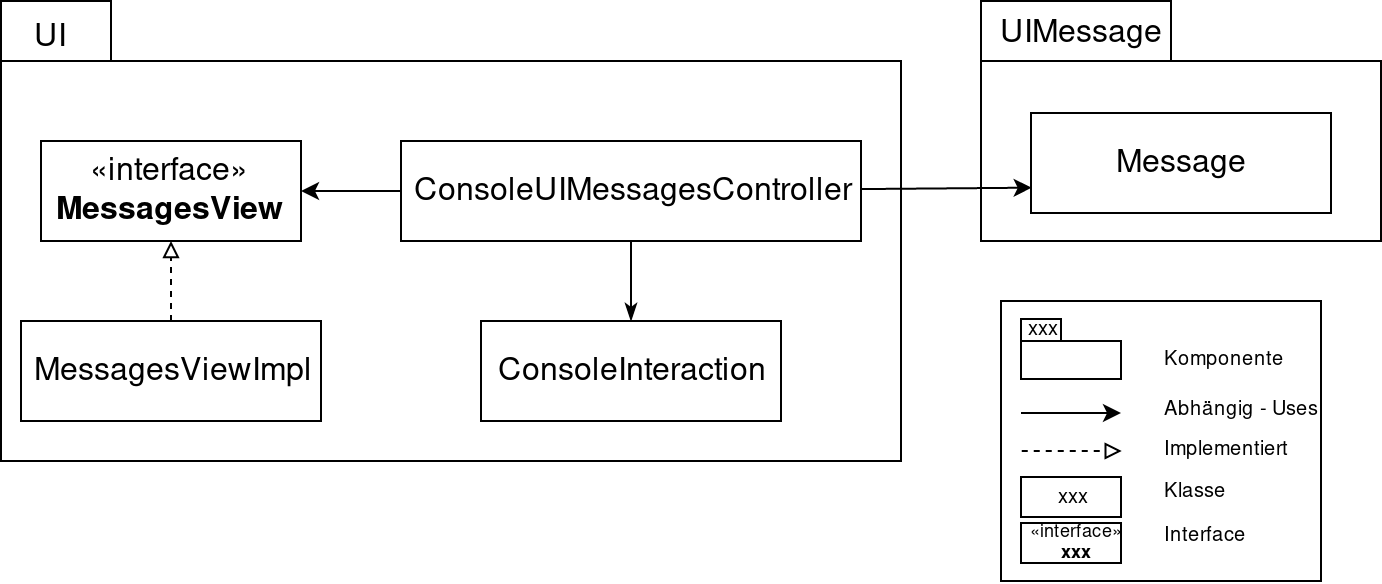
\includegraphics[keepaspectratio,width=\linewidth]{ClassdiagrammUI}
	\caption{Klassendiagramm der Komponente UI mit Darstellung der Abhängigkeit zu UI Message}
	\label{fig:ClassUI}
\end{figure}
\subsubsection{UI Message}

\subsubsection{Misplaced Tag Identifier}
\begin{figure}[htb]
	\centering
	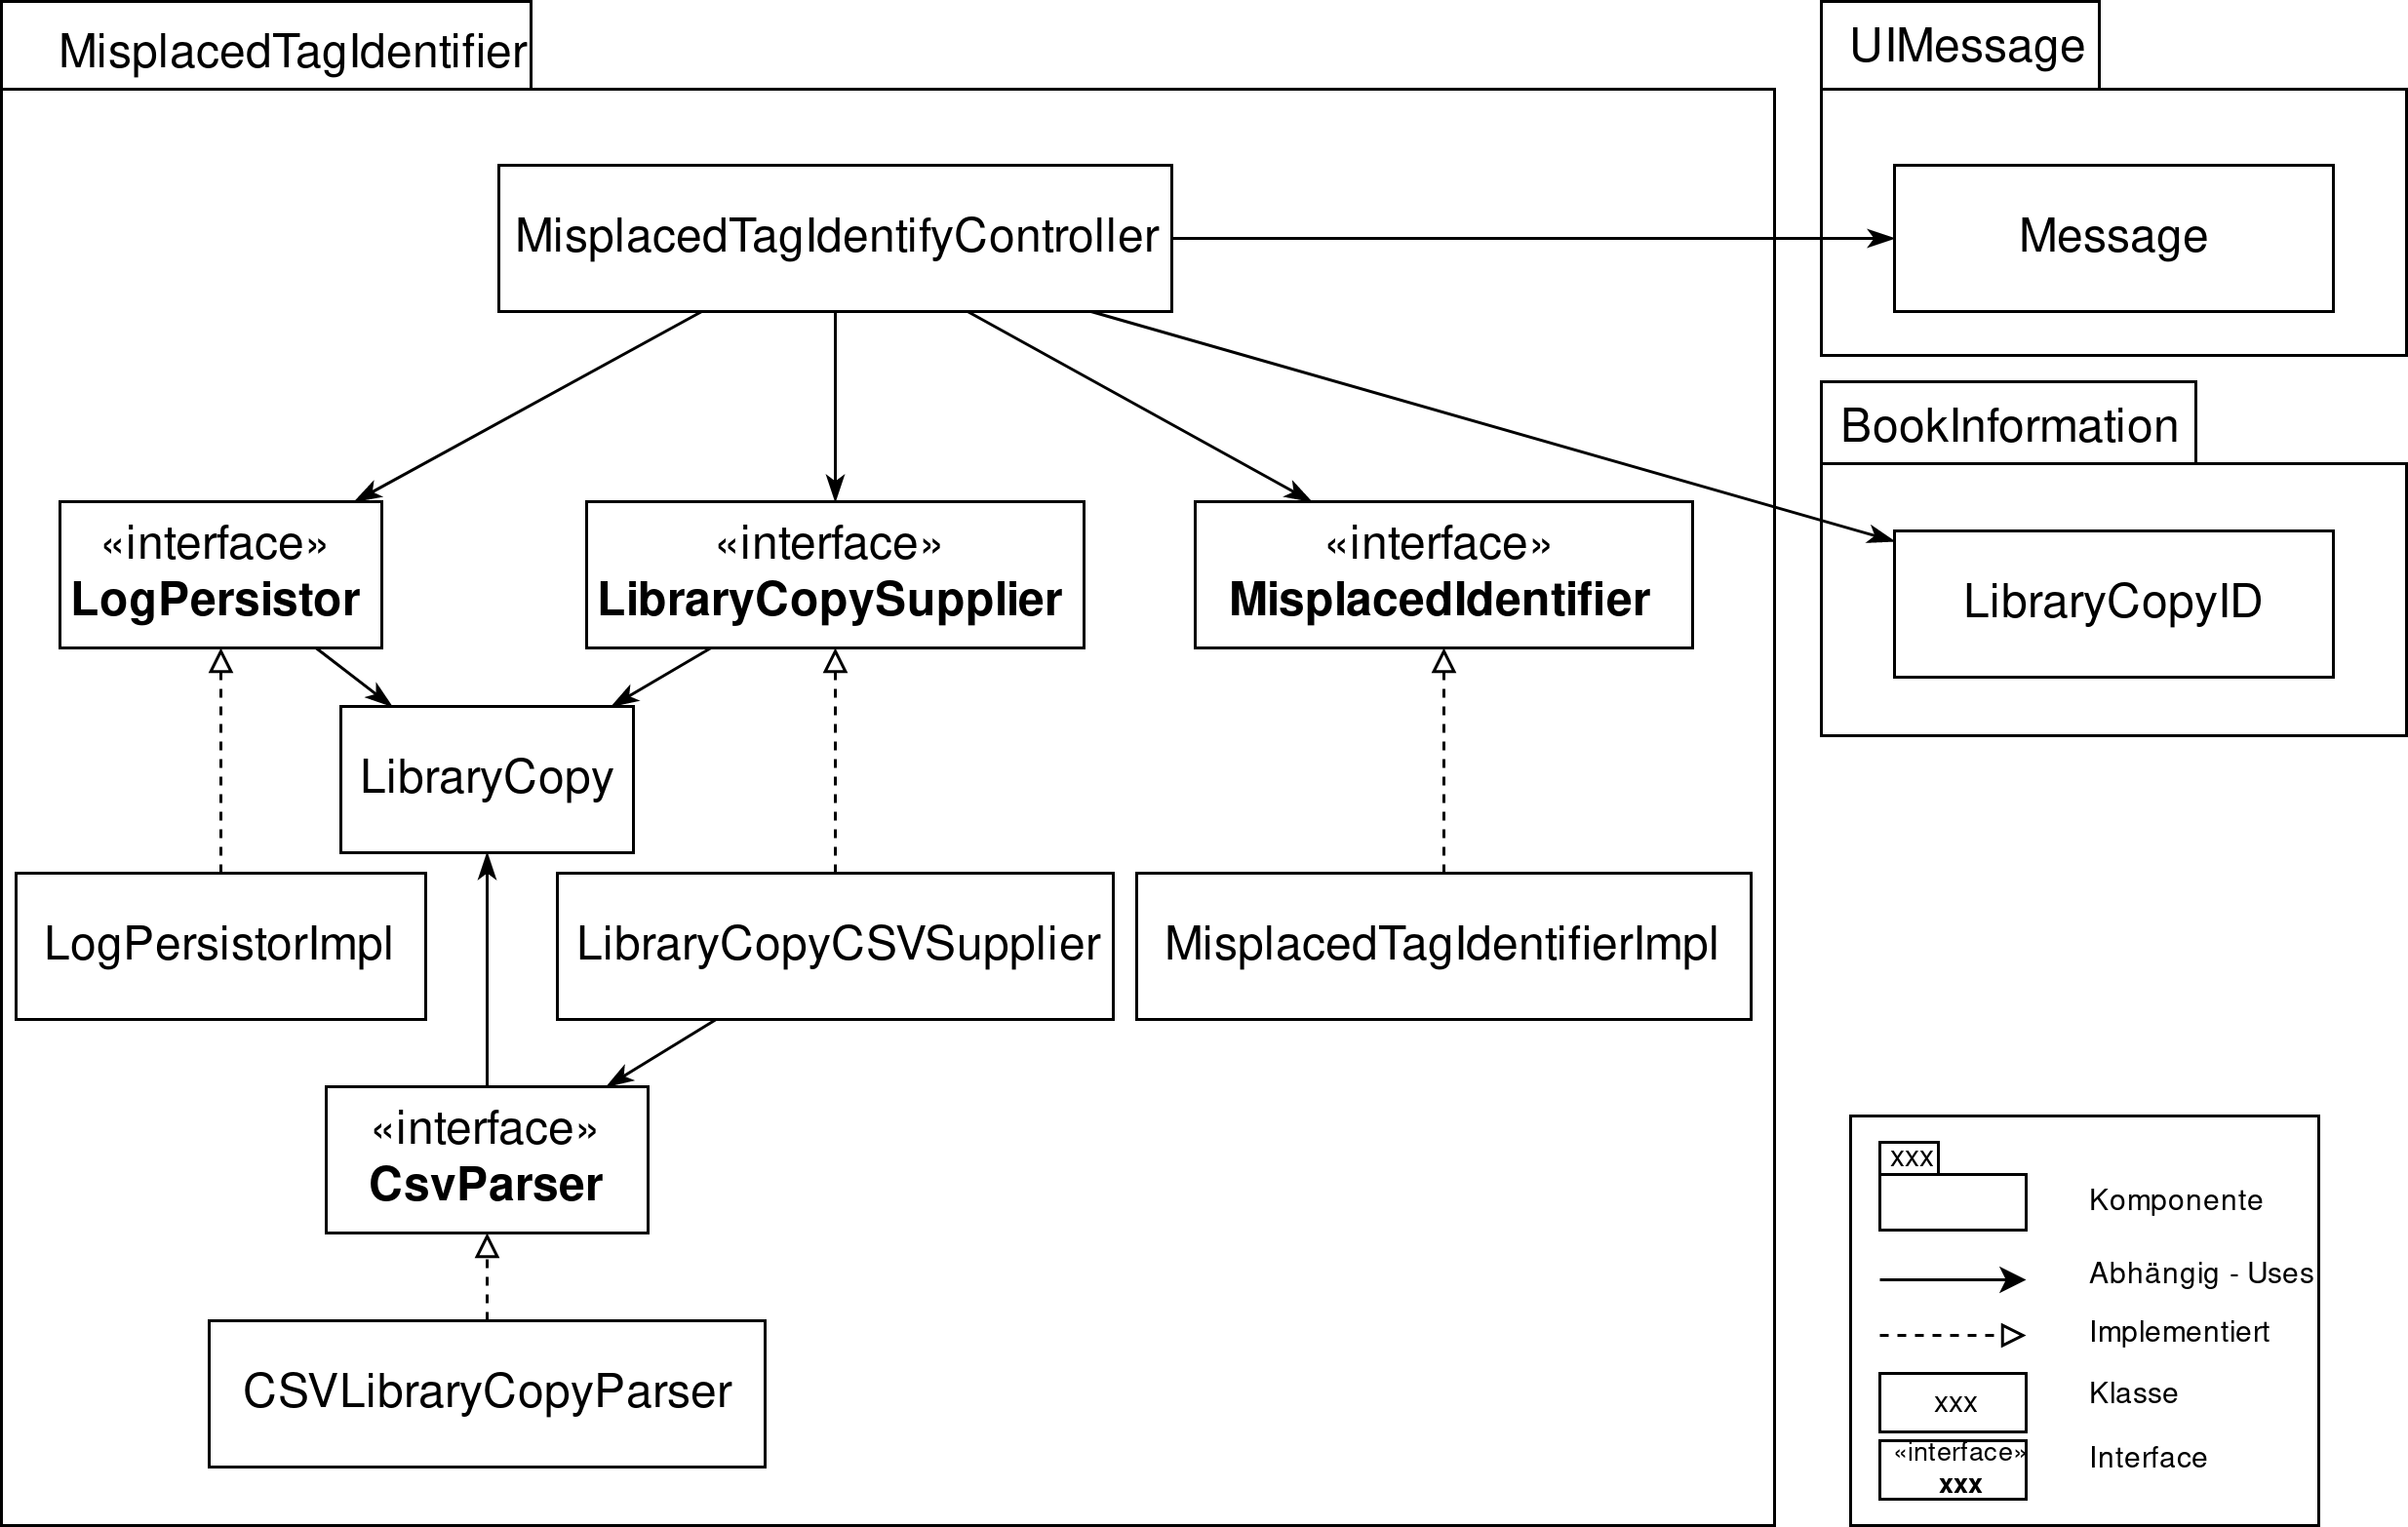
\includegraphics[keepaspectratio,width=\linewidth]{ClassdiagrammMisplacedTagIdentifier}
	\caption{Klassendiagramm der Komponente Misplaced Tag Identifier mit Darstellung der Abhängigkeit zu UI Message und Book Information}
	\label{fig:ClassMisplacedTagIdentifier}
\end{figure}

\subsubsection{Book Information}
\subsubsection{Tag Reader}
\begin{figure}[htb]
	\centering
	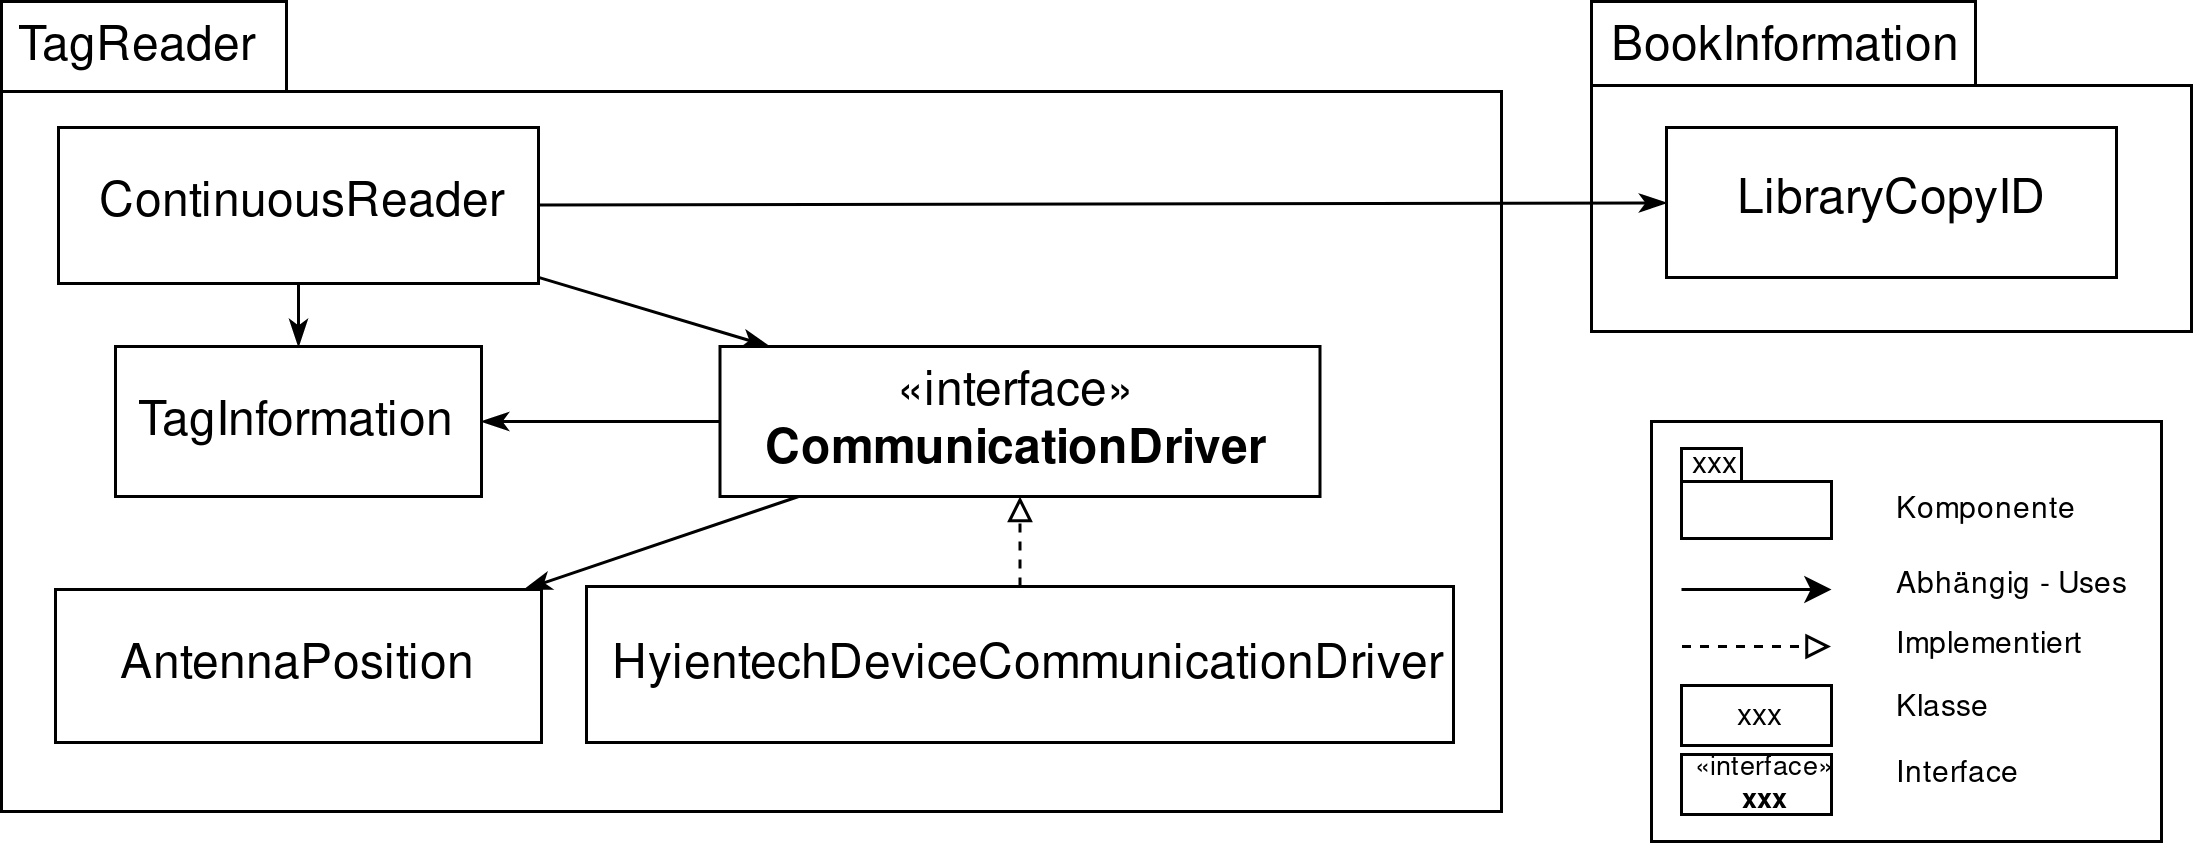
\includegraphics[keepaspectratio,width=\linewidth]{ClassdiagrammTagReader}
	\caption{Klassendiagramm der Komponente Tag Reader mit Darstellung der Abhängigkeit zu Book Information}
	\label{fig:ClassTagReader}
\end{figure}



\subsection{Interne Schnittstellen}

\subsection{Klassendiagramm}

\subsection{Anforderungen der Software}

\subsection{Umsetzung Programmierung}

\subsection{Testing}
